% Created by tikzDevice version 0.12.3.1 on 2022-03-06 11:19:30
% !TEX encoding = UTF-8 Unicode
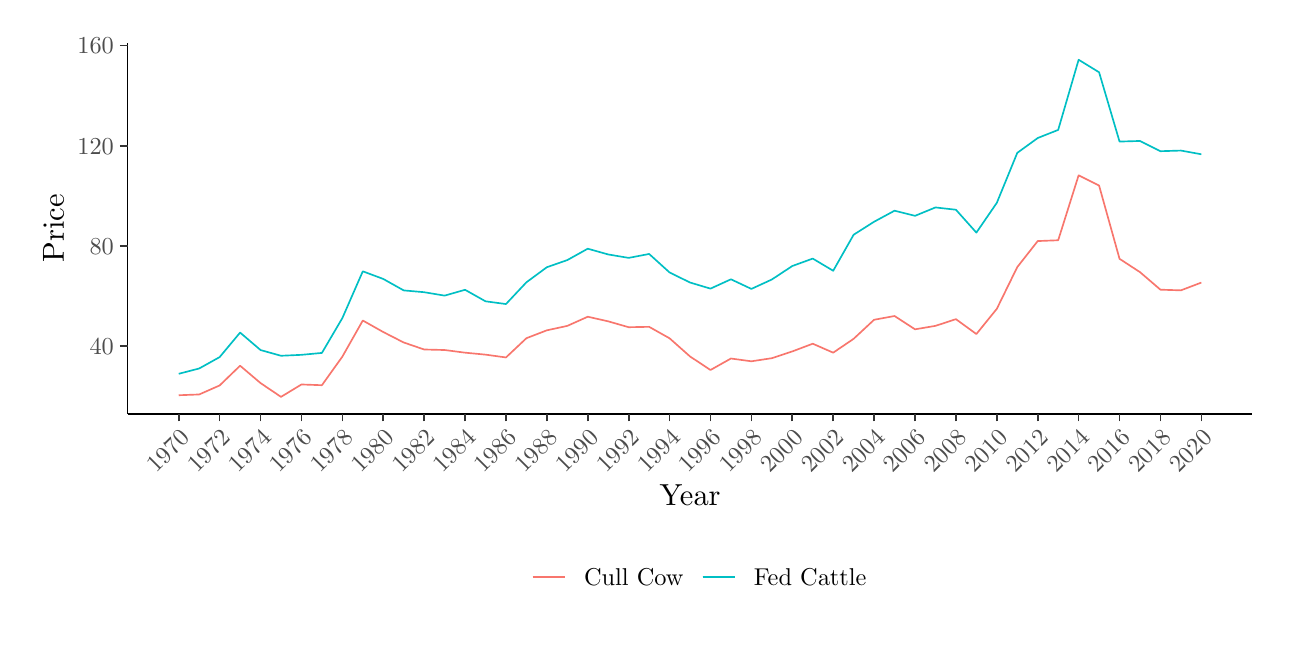
\begin{tikzpicture}[x=1pt,y=1pt]
\definecolor{fillColor}{RGB}{255,255,255}
\path[use as bounding box,fill=fillColor,fill opacity=0.00] (0,0) rectangle (448.07,216.81);
\begin{scope}
\path[clip] (  0.00,  0.00) rectangle (448.07,216.81);
\definecolor{drawColor}{RGB}{255,255,255}
\definecolor{fillColor}{RGB}{255,255,255}

\path[draw=drawColor,line width= 0.6pt,line join=round,line cap=round,fill=fillColor] (  0.00,  0.00) rectangle (448.07,216.81);
\end{scope}
\begin{scope}
\path[clip] ( 36.11, 77.31) rectangle (442.57,211.31);
\definecolor{fillColor}{RGB}{255,255,255}

\path[fill=fillColor] ( 36.11, 77.31) rectangle (442.57,211.31);
\definecolor{drawColor}{RGB}{0,191,196}

\path[draw=drawColor,line width= 0.6pt,line join=round] ( 54.59, 91.74) --
	( 61.98, 93.66) --
	( 69.37, 97.77) --
	( 76.76,106.63) --
	( 84.15,100.32) --
	( 91.54, 98.25) --
	( 98.93, 98.59) --
	(106.32, 99.28) --
	(113.71,111.87) --
	(121.10,128.77) --
	(128.49,126.01) --
	(135.88,121.87) --
	(143.27,121.22) --
	(150.66,119.98) --
	(158.05,122.09) --
	(165.44,117.93) --
	(172.83,116.94) --
	(180.22,124.80) --
	(187.61,130.25) --
	(195.00,132.83) --
	(202.39,136.94) --
	(209.78,134.86) --
	(217.17,133.62) --
	(224.56,135.04) --
	(231.95,128.35) --
	(239.34,124.72) --
	(246.73,122.51) --
	(254.12,125.89) --
	(261.51,122.41) --
	(268.90,125.81) --
	(276.29,130.68) --
	(283.68,133.37) --
	(291.07,128.97) --
	(298.46,141.99) --
	(305.85,146.68) --
	(313.24,150.67) --
	(320.64,148.82) --
	(328.03,151.85) --
	(335.42,151.02) --
	(342.81,142.75) --
	(350.20,153.52) --
	(357.59,171.57) --
	(364.98,176.93) --
	(372.37,179.87) --
	(379.76,205.22) --
	(387.15,200.69) --
	(394.54,175.65) --
	(401.93,175.87) --
	(409.32,172.17) --
	(416.71,172.40) --
	(424.10,171.06);
\definecolor{drawColor}{RGB}{248,118,109}

\path[draw=drawColor,line width= 0.6pt,line join=round] ( 54.59, 83.99) --
	( 61.98, 84.27) --
	( 69.37, 87.53) --
	( 76.76, 94.66) --
	( 84.15, 88.38) --
	( 91.54, 83.40) --
	( 98.93, 87.88) --
	(106.32, 87.61) --
	(113.71, 97.94) --
	(121.10,110.99) --
	(128.49,106.83) --
	(135.88,103.05) --
	(143.27,100.52) --
	(150.66,100.33) --
	(158.05, 99.37) --
	(165.44, 98.66) --
	(172.83, 97.64) --
	(180.22,104.60) --
	(187.61,107.45) --
	(195.00,109.05) --
	(202.39,112.36) --
	(209.78,110.69) --
	(217.17,108.57) --
	(224.56,108.71) --
	(231.95,104.56) --
	(239.34, 98.00) --
	(246.73, 93.11) --
	(254.12, 97.26) --
	(261.51, 96.25) --
	(268.90, 97.38) --
	(276.29, 99.82) --
	(283.68,102.61) --
	(291.07, 99.37) --
	(298.46,104.38) --
	(305.85,111.26) --
	(313.24,112.62) --
	(320.64,107.81) --
	(328.03,109.06) --
	(335.42,111.48) --
	(342.81,106.10) --
	(350.20,115.22) --
	(357.59,130.30) --
	(364.98,139.70) --
	(372.37,139.99) --
	(379.76,163.47) --
	(387.15,159.75) --
	(394.54,133.29) --
	(401.93,128.47) --
	(409.32,122.13) --
	(416.71,121.89) --
	(424.10,124.70);
\end{scope}
\begin{scope}
\path[clip] (  0.00,  0.00) rectangle (448.07,216.81);
\definecolor{drawColor}{RGB}{0,0,0}

\path[draw=drawColor,line width= 0.6pt,line join=round] ( 36.11, 77.31) --
	( 36.11,211.31);
\end{scope}
\begin{scope}
\path[clip] (  0.00,  0.00) rectangle (448.07,216.81);
\definecolor{drawColor}{gray}{0.30}

\node[text=drawColor,anchor=base east,inner sep=0pt, outer sep=0pt, scale=  0.88] at ( 31.16, 98.67) {40};

\node[text=drawColor,anchor=base east,inner sep=0pt, outer sep=0pt, scale=  0.88] at ( 31.16,134.89) {80};

\node[text=drawColor,anchor=base east,inner sep=0pt, outer sep=0pt, scale=  0.88] at ( 31.16,171.11) {120};

\node[text=drawColor,anchor=base east,inner sep=0pt, outer sep=0pt, scale=  0.88] at ( 31.16,207.32) {160};
\end{scope}
\begin{scope}
\path[clip] (  0.00,  0.00) rectangle (448.07,216.81);
\definecolor{drawColor}{gray}{0.20}

\path[draw=drawColor,line width= 0.6pt,line join=round] ( 33.36,101.70) --
	( 36.11,101.70);

\path[draw=drawColor,line width= 0.6pt,line join=round] ( 33.36,137.92) --
	( 36.11,137.92);

\path[draw=drawColor,line width= 0.6pt,line join=round] ( 33.36,174.14) --
	( 36.11,174.14);

\path[draw=drawColor,line width= 0.6pt,line join=round] ( 33.36,210.35) --
	( 36.11,210.35);
\end{scope}
\begin{scope}
\path[clip] (  0.00,  0.00) rectangle (448.07,216.81);
\definecolor{drawColor}{RGB}{0,0,0}

\path[draw=drawColor,line width= 0.6pt,line join=round] ( 36.11, 77.31) --
	(442.57, 77.31);
\end{scope}
\begin{scope}
\path[clip] (  0.00,  0.00) rectangle (448.07,216.81);
\definecolor{drawColor}{gray}{0.20}

\path[draw=drawColor,line width= 0.6pt,line join=round] ( 54.59, 74.56) --
	( 54.59, 77.31);

\path[draw=drawColor,line width= 0.6pt,line join=round] ( 69.37, 74.56) --
	( 69.37, 77.31);

\path[draw=drawColor,line width= 0.6pt,line join=round] ( 84.15, 74.56) --
	( 84.15, 77.31);

\path[draw=drawColor,line width= 0.6pt,line join=round] ( 98.93, 74.56) --
	( 98.93, 77.31);

\path[draw=drawColor,line width= 0.6pt,line join=round] (113.71, 74.56) --
	(113.71, 77.31);

\path[draw=drawColor,line width= 0.6pt,line join=round] (128.49, 74.56) --
	(128.49, 77.31);

\path[draw=drawColor,line width= 0.6pt,line join=round] (143.27, 74.56) --
	(143.27, 77.31);

\path[draw=drawColor,line width= 0.6pt,line join=round] (158.05, 74.56) --
	(158.05, 77.31);

\path[draw=drawColor,line width= 0.6pt,line join=round] (172.83, 74.56) --
	(172.83, 77.31);

\path[draw=drawColor,line width= 0.6pt,line join=round] (187.61, 74.56) --
	(187.61, 77.31);

\path[draw=drawColor,line width= 0.6pt,line join=round] (202.39, 74.56) --
	(202.39, 77.31);

\path[draw=drawColor,line width= 0.6pt,line join=round] (217.17, 74.56) --
	(217.17, 77.31);

\path[draw=drawColor,line width= 0.6pt,line join=round] (231.95, 74.56) --
	(231.95, 77.31);

\path[draw=drawColor,line width= 0.6pt,line join=round] (246.73, 74.56) --
	(246.73, 77.31);

\path[draw=drawColor,line width= 0.6pt,line join=round] (261.51, 74.56) --
	(261.51, 77.31);

\path[draw=drawColor,line width= 0.6pt,line join=round] (276.29, 74.56) --
	(276.29, 77.31);

\path[draw=drawColor,line width= 0.6pt,line join=round] (291.07, 74.56) --
	(291.07, 77.31);

\path[draw=drawColor,line width= 0.6pt,line join=round] (305.85, 74.56) --
	(305.85, 77.31);

\path[draw=drawColor,line width= 0.6pt,line join=round] (320.64, 74.56) --
	(320.64, 77.31);

\path[draw=drawColor,line width= 0.6pt,line join=round] (335.42, 74.56) --
	(335.42, 77.31);

\path[draw=drawColor,line width= 0.6pt,line join=round] (350.20, 74.56) --
	(350.20, 77.31);

\path[draw=drawColor,line width= 0.6pt,line join=round] (364.98, 74.56) --
	(364.98, 77.31);

\path[draw=drawColor,line width= 0.6pt,line join=round] (379.76, 74.56) --
	(379.76, 77.31);

\path[draw=drawColor,line width= 0.6pt,line join=round] (394.54, 74.56) --
	(394.54, 77.31);

\path[draw=drawColor,line width= 0.6pt,line join=round] (409.32, 74.56) --
	(409.32, 77.31);

\path[draw=drawColor,line width= 0.6pt,line join=round] (424.10, 74.56) --
	(424.10, 77.31);
\end{scope}
\begin{scope}
\path[clip] (  0.00,  0.00) rectangle (448.07,216.81);
\definecolor{drawColor}{gray}{0.30}

\node[text=drawColor,rotate= 45.00,anchor=base east,inner sep=0pt, outer sep=0pt, scale=  0.88] at ( 58.87, 68.07) {1970};

\node[text=drawColor,rotate= 45.00,anchor=base east,inner sep=0pt, outer sep=0pt, scale=  0.88] at ( 73.65, 68.07) {1972};

\node[text=drawColor,rotate= 45.00,anchor=base east,inner sep=0pt, outer sep=0pt, scale=  0.88] at ( 88.43, 68.07) {1974};

\node[text=drawColor,rotate= 45.00,anchor=base east,inner sep=0pt, outer sep=0pt, scale=  0.88] at (103.21, 68.07) {1976};

\node[text=drawColor,rotate= 45.00,anchor=base east,inner sep=0pt, outer sep=0pt, scale=  0.88] at (117.99, 68.07) {1978};

\node[text=drawColor,rotate= 45.00,anchor=base east,inner sep=0pt, outer sep=0pt, scale=  0.88] at (132.77, 68.07) {1980};

\node[text=drawColor,rotate= 45.00,anchor=base east,inner sep=0pt, outer sep=0pt, scale=  0.88] at (147.56, 68.07) {1982};

\node[text=drawColor,rotate= 45.00,anchor=base east,inner sep=0pt, outer sep=0pt, scale=  0.88] at (162.34, 68.07) {1984};

\node[text=drawColor,rotate= 45.00,anchor=base east,inner sep=0pt, outer sep=0pt, scale=  0.88] at (177.12, 68.07) {1986};

\node[text=drawColor,rotate= 45.00,anchor=base east,inner sep=0pt, outer sep=0pt, scale=  0.88] at (191.90, 68.07) {1988};

\node[text=drawColor,rotate= 45.00,anchor=base east,inner sep=0pt, outer sep=0pt, scale=  0.88] at (206.68, 68.07) {1990};

\node[text=drawColor,rotate= 45.00,anchor=base east,inner sep=0pt, outer sep=0pt, scale=  0.88] at (221.46, 68.07) {1992};

\node[text=drawColor,rotate= 45.00,anchor=base east,inner sep=0pt, outer sep=0pt, scale=  0.88] at (236.24, 68.07) {1994};

\node[text=drawColor,rotate= 45.00,anchor=base east,inner sep=0pt, outer sep=0pt, scale=  0.88] at (251.02, 68.07) {1996};

\node[text=drawColor,rotate= 45.00,anchor=base east,inner sep=0pt, outer sep=0pt, scale=  0.88] at (265.80, 68.07) {1998};

\node[text=drawColor,rotate= 45.00,anchor=base east,inner sep=0pt, outer sep=0pt, scale=  0.88] at (280.58, 68.07) {2000};

\node[text=drawColor,rotate= 45.00,anchor=base east,inner sep=0pt, outer sep=0pt, scale=  0.88] at (295.36, 68.07) {2002};

\node[text=drawColor,rotate= 45.00,anchor=base east,inner sep=0pt, outer sep=0pt, scale=  0.88] at (310.14, 68.07) {2004};

\node[text=drawColor,rotate= 45.00,anchor=base east,inner sep=0pt, outer sep=0pt, scale=  0.88] at (324.92, 68.07) {2006};

\node[text=drawColor,rotate= 45.00,anchor=base east,inner sep=0pt, outer sep=0pt, scale=  0.88] at (339.70, 68.07) {2008};

\node[text=drawColor,rotate= 45.00,anchor=base east,inner sep=0pt, outer sep=0pt, scale=  0.88] at (354.48, 68.07) {2010};

\node[text=drawColor,rotate= 45.00,anchor=base east,inner sep=0pt, outer sep=0pt, scale=  0.88] at (369.26, 68.07) {2012};

\node[text=drawColor,rotate= 45.00,anchor=base east,inner sep=0pt, outer sep=0pt, scale=  0.88] at (384.04, 68.07) {2014};

\node[text=drawColor,rotate= 45.00,anchor=base east,inner sep=0pt, outer sep=0pt, scale=  0.88] at (398.82, 68.07) {2016};

\node[text=drawColor,rotate= 45.00,anchor=base east,inner sep=0pt, outer sep=0pt, scale=  0.88] at (413.60, 68.07) {2018};

\node[text=drawColor,rotate= 45.00,anchor=base east,inner sep=0pt, outer sep=0pt, scale=  0.88] at (428.38, 68.07) {2020};
\end{scope}
\begin{scope}
\path[clip] (  0.00,  0.00) rectangle (448.07,216.81);
\definecolor{drawColor}{RGB}{0,0,0}

\node[text=drawColor,anchor=base,inner sep=0pt, outer sep=0pt, scale=  1.10] at (239.34, 44.09) {Year};
\end{scope}
\begin{scope}
\path[clip] (  0.00,  0.00) rectangle (448.07,216.81);
\definecolor{drawColor}{RGB}{0,0,0}

\node[text=drawColor,rotate= 90.00,anchor=base,inner sep=0pt, outer sep=0pt, scale=  1.10] at ( 13.08,144.31) {Price};
\end{scope}
\begin{scope}
\path[clip] (  0.00,  0.00) rectangle (448.07,216.81);
\definecolor{fillColor}{RGB}{255,255,255}

\path[fill=fillColor] (170.08,  5.50) rectangle (308.60, 30.95);
\end{scope}
\begin{scope}
\path[clip] (  0.00,  0.00) rectangle (448.07,216.81);
\definecolor{drawColor}{RGB}{248,118,109}

\path[draw=drawColor,line width= 0.6pt,line join=round] (182.53, 18.23) -- (194.09, 18.23);
\end{scope}
\begin{scope}
\path[clip] (  0.00,  0.00) rectangle (448.07,216.81);
\definecolor{drawColor}{RGB}{248,118,109}

\path[draw=drawColor,line width= 0.6pt,line join=round] (182.53, 18.23) -- (194.09, 18.23);
\end{scope}
\begin{scope}
\path[clip] (  0.00,  0.00) rectangle (448.07,216.81);
\definecolor{drawColor}{RGB}{0,191,196}

\path[draw=drawColor,line width= 0.6pt,line join=round] (243.91, 18.23) -- (255.47, 18.23);
\end{scope}
\begin{scope}
\path[clip] (  0.00,  0.00) rectangle (448.07,216.81);
\definecolor{drawColor}{RGB}{0,191,196}

\path[draw=drawColor,line width= 0.6pt,line join=round] (243.91, 18.23) -- (255.47, 18.23);
\end{scope}
\begin{scope}
\path[clip] (  0.00,  0.00) rectangle (448.07,216.81);
\definecolor{drawColor}{RGB}{0,0,0}

\node[text=drawColor,anchor=base west,inner sep=0pt, outer sep=0pt, scale=  0.88] at (201.04, 15.20) {Cull Cow};
\end{scope}
\begin{scope}
\path[clip] (  0.00,  0.00) rectangle (448.07,216.81);
\definecolor{drawColor}{RGB}{0,0,0}

\node[text=drawColor,anchor=base west,inner sep=0pt, outer sep=0pt, scale=  0.88] at (262.41, 15.20) {Fed Cattle};
\end{scope}
\end{tikzpicture}
